%!TEX root = ../dissertation.tex


\chapter{Ensemble}
\label{ensemble}



%!TEX root = ../dissertation.tex


\section{Ensemble Data}
\label{edata}




\subsection{Ensemble Forecasts}
\label{emodel}

As discussed at the beginning of \mbox{chapter \ref{deterministic}}, in order to develop a statistical post-processing method for calibration of numerical weather prediction forecasts, both forecasts and observations must be readily available.
Unfortunately, as mentioned in the Introduction, ``\dots there is a limited database of forecasts for RCEs, making robust statistical techniques difficult\dots''
As limited as databases of deterministic CAM forecasts are, the availability of \emph{ensembles} of CAM forecasts is even worse.


Similar to CAM forecasts, most storm-scale ensemble forecast systems\footnote{The phrase storm-scale ensemble forecast is typically used in reference to ensembles composed of numerical forecasts produced without using cumulus parameterization.} (SSEF) have been erected on a temporary basis, produced in support of various field programs and experiments.
The makeup of these SSEFs are often modified from one program to the next to adapt to the changing needs of the various experiments.
Long running, consistent configured SSEFs were not available for this work.
It is worth noting that as this work neared completion, the Air Force Weather Agency began running an operational SSEF.


One of the largest collections of SSEF forecasts has been produced by the University of Oklahoma's Center for the Analysis and Prediction of Storms (CAPS).
Since 2007, CAPS has been producing CAM forecasts in support of the Hazardous Weather Testbed's (HWT) annual Spring Forecast Experiment (SFE).
From 2007 through 2010, the ensemble configuration changed from year-to-year based on the results of previous years and updated to the WRF modeling system.
In 2010, CAPS produced a 26 member SSEF.
This SSEF was multi-model in nature, initialized at 00 UTC, used 4 km grid spacing, and integrated out to 30 hours.
Of the 26 members, 19 were WRF-ARW\footnote{Weather Research and Forecasting -- Advanced Research WRF} \citep{WRFV3}, 5 were WRF-NMM\footnote{Weather Research and Forecasting -- nonhydrostatic Mesoscale Model} \citep{NAMnWRF-NMM}, and 2 were ARPS\footnote{Advanced Regional Prediction System} \citep{ARPS}.
In 2011, CAPS expanded the SSEF from 26 members to 50, of which 41 were WRF-ARW, 5 were WRF-NMM, and 4 were ARPS.
These forecasts were also initialized at 00 UTC, used a grid spacing of 4 km, but were integrated forward to 36 hours instead of 30.


For this thesis, fifteen members were chosen from the 2010 and 2011 ensembles because these members were configured almost identically between the two years.
These 15 members were composed of 10 WRF-ARW forecasts, 4 WRF-NMM forecasts, and 1 ARPS forecast.
The background initial conditions for these 15 members were downscaled from the 00 UTC 12 km NAM, with additional information coming from a three dimensional variational and cloud analysis from ARPS.
Except for the control members (one each from the WRF-ARW, WRF-NMM, and ARPS), these initial conditions were then perturbed using mesoscale atmospheric perturbations from NOAA's Environmental Modeling Center's operational Short-Range Ensemble Forecast (SREF) system.
Lateral boundary conditions for the three control members came from the 00 UTC NAM forecasts, whereas the remaining 12 members used the SREF forecast corresponding to the perturbations used in the initial conditions.
A listing of the configurations for each member of the SSEF can be found in \mbox{Table \ref{ensemble_members}}.


The only controlled change between 2010 and 2011 for the aforementioned set of 15 forecasts came from a change in the version of WRF. In 2010, \mbox{WRF Version 3.1.1} was used whereas \mbox{WRF Version 3.2.1} was used in 2011.
Changes in the NAM and SREF, which were used for initial and lateral boundary conditions, were controlled by the NOAA National Weather Service and could not be avoided.


In 2010 the HWT SFE ran from 17 May through 18 June, and in 2011, the HWT SFE ran from 09  May through 10 June.
CAPS provided SSEF forecasts each weekday during the experiment, with an additional two retrospective forecasts in 2011: one for the 27 April 2011 tornado outbreak in the southeast United States and another for the 22 May 2011 Joplin, Missouri EF-5 tornado.
\mbox{Table \ref{sfedtes}} lists the dates for which CAPS forecasts are available.


In an effort to be consistent with the evaluation carried out on the NSSL-WRF, the decision was made to use six-hour accumulation periods for the SSEF forecasts\footnote{Unless otherwise noted, from this point forward the phrase ``SSEF'', ``SSEF forecasts'', or variants thereof refer to the 15 numerical forecasts that are presented in \mbox{Table \ref{ensemble_members}}.} and the Stage IV analyses.
As was the case with the NSSL-WRF, the SSEF forecasts were drawn from subsets of the \mbox{12-36 hr} forecast period ending at 18, 00, 06, and 12 UTC, but only for \mbox{6 hr} time periods for which every member was available.
Because the 2010 SSEF was only integrated out to \mbox{30 hr}, the potential dataset was immediately reduced to 156 six-hour time periods (52 days times 3 periods a day).




\subsection{Observations}
\label{eobservations}

As was the case for the evaluating the deterministic model calibration, NCEP's Stage IV national quantitative precipitation estimate analysis was chosen as the verification dataset.
Please see \mbox{section \ref{observations}} for a description of the Stage IV dataset.




\subsection{Processing}
\label{eprocessing}

As stated in \mbox{section \ref{emodel}}, there were a maximum of 156 six-hour time periods for which SSEF data was expected.
This potential dataset was further thinned by removing all time periods in which either one or more SSEF members were missing or the Stage IV analysis was unavailable.
An additional 37 six-hour time periods were removed as a result, leaving 119 six-hour time periods, over 2010 and 2011, for which both the entire SSEF and the Stage IV analyses are available.


Next, as was necessary with the deterministic forecasts, the ensemble forecasts were interpolated to the Stage IV grid.
All diagnostics and analyses were conducted on this grid.
Furthermore, the same mask shown in \mbox{Figure \ref{domain}} was used to limit the analyses to areas east of the Rocky Mountains and near land.


Unfortunately, 119 time periods is a very small sample from which to evaluate a method for statical calibration of forecasts of rare events.
This is especially true when the training and forecast data must both come from the 119 time periods.
For comparison, the NSSL-WRF training dataset had 4120 training time periods and 1425 forecast time periods.
In an attempt to maximize the utility of the 119 time periods, twenty ``simulations'' were created by resampling the 119 time periods.
This was accomplished by randomly drawing, without replacement, 59 training periods from the valid 119 time periods with the remaining 60 periods used as forecast periods.
From these 59 training periods, two-dimensional histograms were created for each of the 15 ensemble members.
These histograms were then used to calculate the five fitting parameters --- $\sigma_x$, $\sigma_y$, $\theta$, $h$, and $k$ --- for each member's unique two-dimensional anisotropic Gaussian function.
Forecasts for each member were then made for each time period of the 60 forecast time periods, with each member using its own fitted anisotropic Gaussian function.
Thus, for each simulation all 15 ensemble members used the same 59 time periods for training and the remaining 60 time periods for forecasting.
This results in 18 000 forecasts (20 simulations x 60 forecast periods x 15 members).







%!TEX root = ../dissertation.tex


\section{Ensemble Results}
\label{eresults}




\subsection{25.4 mm Threshold}
\label{eresults_25.4mm}

As previously mentioned, the first step of the proposed calibration process is to create two-dimensional composites of where observations occurred relative to forecast grid points.
In the case of the small number of SSEF forecasts, this amounts to creating a composite for each member for each simulation.
\mbox{Figure \ref{ssef-25mm-400km-composite}} shows the the two-dimensional composites for each member at the \mbox{25.4 mm} in \mbox{6 hr} threshold for one of the twenty simulations.
In this simulation, it is readily apparent that the WRF-NMM ensemble members are generaly the wettest, with the WRF-ARW members drier.
(The ARPS member is in between.)
The overall axis of observations relative to forecasts indicates a general southeast-to-northeast orientation in most members, although this is more readily apparent in some members than others.


Although the orientation of the axis of maximum observations tends to generally be similar between members, the centroid of the distribution exhibits more variability.
About half of the members have the centroid of observations too far east and half having the centroid be too far west.
(This corresponds to the $h$ parameter of the Gaussian fitting parameters.)
The members having the observations centroid too far east tended to be farther away from the forecast than those members having the observations centroid too far west.
In this simulation, the WRF-NMM has a westward bias with its forecasts, as the centroid of observations is east of the forecast grid point in every WRF-NMM member.
A similar observation cannot be made for the WRF-ARW members.
It is unclear from this single simulation if the westward forecast bias in the WRF-NMM members is systematic of the WRF-NMM core, or merely a function of only having 4 WRF-NMM members.


When examining the north/south variations of the observations centroid relative to the model forecast, similar variations are observed.
(The north/south displacement of the observations centroid corresponds to the $k$ parameter of the Gaussian fitting parameters.)
Slightly more than half the members have the centroid of observations too far north, indicating a southward bias of the forecast, with slightly less than half having the centroid of observations too far south.
Three of the four WRF-NMM members had the forecast too far north, with the WRF-NMM control member having the greatest displacement.
No obvious preference in displacement direction is readily apparent from the WRF-ARW members.
However, it does appear that generally speaking, the magnitude of the displacement of the WRF-ARW members appears to be less than that of the WRF-NMM members.


The lower right panel of \mbox{Figure \ref{ssef-25mm-400km-composite}} depicts the standard deviation between the two-dimensional composites of each member for the given simulation.
In this panel, the darker colors indicate a greater standard deviation at that particular grid point than grid points with a lighter color.
It is readily apparent that the greatest variability between the members exists to the east of the forecast grid point.
This is due to the wetter WRF-NMM members having a westward forecast bias, resulting in a wider range of observation counts to the east of the forecast.


Unfortunately, \mbox{Figure \ref{ssef-25mm-400km-composite}} is only one simulation out of the twenty simulations produced.
In an attempt to gain insights into the variation of the two-dimensional composites for each member between all twenty simulations, the standard deviation of each member's composites is shown in \mbox{Figure \ref{ssef-25mm-400km-std}}.
A cursory examination of the standard deviation of the two-dimensional composites does not yield any immediate insights.
Some members exhibit a maximum in variability along a southwest to northeast orientation.
Other members exhibit a more uniform increase in the maximum variability.
In both cases, the maximum variability tended to be located near the forecast grid point, with generally decreasing variability as distance from the forecast grid point increases.


Breaking down the fitting parameters by simulation gives an even better idea of the variability in each member's twenty two-dimensional composites.
A set of five figures (\mbox{Figures \ref{sigmax-25mm-400km-dist}--\ref{k-25mm-400km-dist}}) were created to examine the variability of each of the five Gaussian fitting parameters --- one figure per fitting parameter.
The figures contain box-and-whisker plots for each member's distribution of that figure's fitting parameter.
The box-and-whisker plots offer insight into the variability in the various fitting functions used by each member.
In each of the figures, the red horizontal line marks the median value of the distributions, and the blue box represents the 25th and 75th percentiles.
The whiskers denote the range of the distribution, up to $\pm$ 1.5 times the interquartile range.
Gold stars are used to denote any outliers, defined to be any value of the distribution that is outside the range of $\pm$ 1.5 times the interquartile range.


\mbox{Figure \ref{sigmax-25mm-400km-dist}} displays the box-and-whisker plots for the $\sigma_x$ fitting parameter.
This parameter is the length of the long axis of the fitted anisotropic Gaussian function.
Nine out of the fifteen ensemble members do not have outliers.
Of the remaining six ensemble members with outliers, two of them only have one outlier, two of them have two outliers, and one each has four and five outliers.
Ensemble members that have outliers had a range of over 20 kilometers for $\sigma_x$, whereas those members without outliers generally had ranges of less than 20 kilometers.
This means that 40\% of the ensemble members had variability in their $\sigma_x$ parameter that was greater than 10\% of the median length of the $\sigma_x$ fitting parameter.


\mbox{Figure \ref{sigmay-25mm-400km-dist}} shows the box-and-whisker plots for the $\sigma_y$ fitting parameter.
This parameter is the length of the short axis of the fitted anisotropic Gaussian function.
Unlike with the $\sigma_x$ fitting parameter, the ensemble member distributions of the $\sigma_y$ fitting parameter exhibit fewer outliers with only four members having them.
This can be attributed to their being more variability in the 25th to 75th percentile, as noted by the increased size of the boxes for many members.
Furthermore, whereas when the maximum range of the $\sigma_x$ fitting parameter distribution greater than 20 kilometers indicated the presence of an outlier, several members have distributions of $\sigma_y$ with a maximum range greater than 20 kilometers without having an outlier.
In fact, six out of the ten WRF-ARW members have a range of $\sigma_y$ greater than 20 kilometers and only two of them have outliers.


The distributions of the counter-clockwise rotation angle of the abscissa, fitting parameter $\theta$, is shown in \mbox{Figure \ref{theta-25mm-400km-dist}}.
For this fitting parameter, eleven out of fifteen members exhibit outliers.
This is not really surprising when one considers the overlap in the distributions of fitting parameters $\sigma_x$ and $\sigma_y$.
As alluded to in \mbox{Section \ref{std}}, when $\sigma_x$ approaches $\sigma_y$, the Gaussian function approaches being isotropy.
As a Gaussian function approaches isotropy the variability of the rotation angle, $\theta$ increases as a result of the more circular nature to the function.
It is much more difficult to accurately measure the orientation of the rotation angle of an ellipse that is nearly circular than that of one with a high level of eccentricity.


The variability in the fitting parameters was not limited to just the shape of the anisotropic Gaussian.
The location of the fitting Gaussian also ranged widely.
Each member's distributions of the $h$ fitting parameter (displacement in the east or west direction) is shown in \mbox{Figure \ref{h-25mm-400km-dist}}.
Generally speaking, some of the values for $h$ deviated from the forecast grid point by over 40 kilometers.
The ARPS and WRF-NMM members consistently demonstrated a bias toward the observations centroid being east.
This corresponds to the forecasts, on average, being too far west compared to where observations occurred.
Most of the WRF-ARW members exhibited the opposite behavior, namely having the observations being too far east (indicating an eastward bias with the forecast).
Not every WRF-ARW member exhibited this bias, however.
The values comprising the interquartile range for two of the WRF-ARW members consisted of positive values for $h$, indicating a westward forecast bias.
However, unlike with the ARPS and WRF-NMM members, where the entire distribution consisted of positive values for $h$, every member of the WRF-ARW had at least a portion of the ``whiskers'' part of the box-and whiskers plot with negative values, indicating an eastward forecast bias, as compared to observations.



















% table definitions
%%%%%%%%%%%%%%%%%%%
\newenvironment{telement}[2]{\begin{minipage}[c]{#1} \centering #2} {\end{minipage}}
\newcommand{\coremem}{\color{black}}
\newcommand{\member}[1]{\begin{telement}{0.75in}{#1}\end{telement}}
\newcommand{\ic}[1]{\begin{telement}{1in}{#1}\end{telement}}
\newcommand{\bc}[1]{\begin{telement}{0.75in}{#1}\end{telement}}
\newcommand{\radar}[1]{\begin{telement}{0.75in}{#1}\end{telement}}
\newcommand{\microphysics}[1]{\begin{telement}{0.75in}{#1}\end{telement}}
\newcommand{\lsm}[1]{\begin{telement}{0.75in}{#1}\end{telement}}
\newcommand{\pbl}[1]{\begin{telement}{0.75in}{#1}\end{telement}}

\newpage

\begin{center}
    \renewcommand{\arraystretch}{3}
    \centering
    \singlespace
    \small
    \setlength\tabcolsep{2pt}
    \rowcolors{2}{gray!20}{white}
    \begin{longtable}{|c|c|c|c|c|c|c|}
        \caption[Configurations for the 2010 and 2011 CAPS Ensemble Members]
        {Configurations for the 2010 and 2011 CAPS Ensemble Members.}
        \label{ensemble_members} \\

        % Header for the first page
        \hline
        \rowcolor{gray!60}
        \member{\textbf{Member}} &
        \ic{\textbf{I. C.}} &
        \bc{\textbf{B. C.}} &
        \radar{\textbf{Radar}} &
        \microphysics{\textbf{Micro-\\physics}} &
        \lsm{\textbf{LSM}} &
        \pbl{\textbf{PBL}} \\
        \hline
        \endfirsthead

        % Header for remaining pages
        \hline
        \multicolumn{7}{|c|}{{\tablename} \thetable{} -- Continued} \\
        \hline
        \rowcolor{gray!60}
        \member{\textbf{Member}} &
        \ic{\textbf{I. C.}} &
        \bc{\textbf{B. C.}} &
        \radar{\textbf{Radar}} &
        \microphysics{\textbf{Micro-\\physics}} &
        \lsm{\textbf{LSM}} &
        \pbl{\textbf{PBL}} \\
        \hline
        \endhead

        %This is the footer for all pages except the last page of the table...
        \multicolumn{7}{|c|}{{Continued on Next Page \ldots}} \\
        \hline
        \endfoot

        %This is the footer for the last page of the table...
        \hline
        \multicolumn{7}{|l|}{Note 1: For all members, cumulus parameterization is turned off} \\
        \hline
        \multicolumn{7}{|l|}{\multirow{1}{\textwidth}{Note 2: For all ARW members, the long-wave radiation parameterization is RRTM and the short-wave radiation parameterization is Goddard}} \\
        \hline
        \multicolumn{7}{|l|}{\multirow{1}{\textwidth}{Note 3: For nmm\_cn, nmm\_m2, \& nmm\_m3 the long-wave radiation parameterization is GFDL and the short-wave radiation parameterization is GFDL}} \\
        \hline
        \multicolumn{7}{|l|}{\multirow{1}{\textwidth}{Note 4: For nmm\_m4 \& nmm\_m5 the long-wave radiation parameterization is RRTM and the short-wave radiation parameterization is Dudhia}}\\
        \hline
        \multicolumn{7}{|l|}{Note 5: The arps member uses Chou/Suarex for radiation} \\
        \hline
        \multicolumn{7}{|l|}{Note 6: Ferrier+ refers to a subset of changes in the updated version now in NEMS/NMMB} \\
        \hline
        \multicolumn{7}{|l|}{\multirow{1}{\textwidth}{Note 7: The ARPS PBL scheme \citep{Xue1996, Sun1986} uses a non-local vertical mixing length within the convective boundary layer}} \\
        \hline
        \endlastfoot

        % Member 1 of 24
        \hline
        \coremem\member{arw\_cn} &
        \coremem\ic{00Z ARPS 3DVAR \& Cloud Analysis} &
        \coremem\bc{00Z NAM Forecast} &
        \coremem\radar{Yes} &
        \coremem\microphysics{Thompson} &
        \coremem\lsm{Noah} &
        \coremem\pbl{MYJ} \\

        % Member 2 of 24
        \hline
        \coremem\member{arw\_m4} &
        \coremem\ic{arw\_cn + em\_p1\_pert} &
        \coremem\bc{21Z SREF em\_p1} &
        \coremem\radar{Yes} &
        \coremem\microphysics{Morrison} &
        \coremem\lsm{RUC} &
        \coremem\pbl{YSU} \\

        % Member 3 of 24
        \hline
        \coremem\member{arw\_m5} &
        \coremem\ic{arw\_cn + em\_p2\_pert} &
        \coremem\bc{21Z SREF em\_p2} &
        \coremem\radar{Yes} &
        \coremem\microphysics{Thompson} &
        \coremem\lsm{Noah} &
        \coremem\pbl{QNSE} \\

        % Member 4 of 24
        \hline
        \coremem\member{arw\_m6} &
        \coremem\ic{arw\_cn - nmm\_p1\_pert} &
        \coremem\bc{21 SREF nmm\_p1} &
        \coremem\radar{Yes} &
        \coremem\microphysics{WSM6} &
        \coremem\lsm{RUC} &
        \coremem\pbl{QNSE} \\

        % Member 5 of 24
        \hline
        \coremem\member{arw\_m7} &
        \coremem\ic{arw\_cn + nmm\_p2\_pert} &
        \coremem\bc{21Z SREF nm\_p2} &
        \coremem\radar{Yes} &
        \coremem\microphysics{WDM6} &
        \coremem\lsm{Noah} &
        \coremem\pbl{MYNN} \\

        % Member 6 of 24
        \hline
        \coremem\member{arw\_m8} &
        \coremem\ic{arw\_cn + rsm\_n1\_pert} &
        \coremem\bc{21Z SREF rsm\_n1} &
        \coremem\radar{Yes} &
        \coremem\microphysics{Ferrier} &
        \coremem\lsm{RUC} &
        \coremem\pbl{YSU} \\

        % Member 7 of 24
        \hline
        \coremem\member{arw\_m9} &
        \coremem\ic{arw\_cn - etaKF\_n1\_pert} &
        \coremem\bc{21Z SREF etaKF\_n1} &
        \coremem\radar{Yes} &
        \coremem\microphysics{Ferrier} &
        \coremem\lsm{Noah} &
        \coremem\pbl{YSU} \\

        % Member 8 or 24
        \hline
        \coremem\member{arw\_m10} &
        \coremem\ic{arw\_cn + etaKF\_p1\_pert} &
        \coremem\bc{21Z SREF etaKF\_p1} &
        \coremem\radar{Yes} &
        \coremem\microphysics{WDM6} &
        \coremem\lsm{Noah} &
        \coremem\pbl{QNSE} \\

        % Member 9 of 24
        \hline
        \coremem\member{arw\_m11} &
        \coremem\ic{arw\_cn - etaBMJ\_p1\_pert} &
        \coremem\bc{21Z SREF etaBMJ\_p1 } &
        \coremem\radar{Yes} &
        \coremem\microphysics{WSM6} &
        \coremem\lsm{RUC} &
        \coremem\pbl{MYNN} \\

        % Member 10 of 24
        \hline
        \coremem\member{arw\_m12} &
        \coremem\ic{arw\_cn + etaBMJ\_p1\_pert} &
        \coremem\bc{21Z SREF etaBMJ\_p1} &
        \coremem\radar{Yes} &
        \coremem\microphysics{Thompson} &
        \coremem\lsm{RUC} &
        \coremem\pbl{MYNN} \\

        % Member 19 of 24
        \hline
        \coremem\member{nmm\_cn} &
        \coremem\ic{00Z ARPS 3DVAR \& Cloud Analysis} &
        \coremem\bc{00Z NAM Forecast} &
        \coremem\radar{Yes} &
        \coremem\microphysics{Ferrier} &
        \coremem\lsm{Noah} &
        \coremem\pbl{MYJ} \\

        % Member 21 of 24
        \hline
        \coremem\member{nmm\_m3} &
        \coremem\ic{nmm\_cn + nmm\_n1\_pert} &
        \coremem\bc{21Z SREF nmm\_n1} &
        \coremem\radar{Yes} &
        \coremem\microphysics{Thompson} &
        \coremem\lsm{Noah} &
        \coremem\pbl{MYJ} \\

        % Member 22 of 24
        \hline
        \coremem\member{nmm\_m4} &
        \coremem\ic{arw\_cn + nmm\_n2\_pert} &
        \coremem\bc{21Z SREF nmm\_n2} &
        \coremem\radar{Yes} &
        \coremem\microphysics{WSM6} &
        \coremem\lsm{RUC} &
        \coremem\pbl{MYJ} \\

        % Member 23 of 24
        \hline
        \coremem\member{nmm\_m5} &
        \coremem\ic{arw\_cn + em\_n1\_pert} &
        \coremem\bc{21Z SREF em\_n1} &
        \coremem\radar{Yes} &
        \coremem\microphysics{Ferrier} &
        \coremem\lsm{RUC} &
        \coremem\pbl{MYJ} \\

        % Member 24 or 24
        \hline
        \coremem\member{arps\_cn} &
        \coremem\ic{00Z ARPS 3DVAR \& Cloud Analysis} &
        \coremem\bc{00Z NAM Forecast} &
        \coremem\radar{Yes} &
        \coremem\microphysics{Lin} &
        \coremem\lsm{Force Restore} &
        \coremem\pbl{1.5-order TKE-based} \\
        \hline

    \end{longtable}
\end{center}




\begin{table}[cc]
    \centering
    \setlength{\tabcolsep}{0.5in}
    \renewcommand{\arraystretch}{1.25}
    \caption[2010 and 2011 dates where CAPS forecasts are available.]
    {2010 and 2011 dates where CAPS forecasts are available.}
    \label{sfedtes} \vspace{0.25in}
    \begin{tabular}{||c c||}
        \hline \hline
        \vspace{\baselineskip} & \vspace{\baselineskip} \\
        \multicolumn{2}{||c||}{\Large 2010 Dates} \\
        \vspace{\baselineskip} & \vspace{\baselineskip} \\
        Week \#1: & 17--21 May 2010 \\
        Week \#2: & 24--28 May 2010 \\
        Week \#3: & 31 May -- 04 June 2010 \\
        Week \#4: & 07--11 June 2010 \\
        Week \#5: & 14--18 June 2010 \\
        \vspace{\baselineskip} & \vspace{\baselineskip} \\
        \hline
        \vspace{\baselineskip} & \vspace{\baselineskip} \\
        \multicolumn{2}{||c||}{\Large 2011 Dates} \\
        \vspace{\baselineskip} & \vspace{\baselineskip} \\
        Week \#1: & 09--13 May 2011 \\
        Week \#2: & 16--20 May 2011 \\
        Week \#3: & 23--27 May 2011 \\
        Week \#4: & 30 May -- 03 June 2011 \\
        Week \#5: & 06--10 June 2011 \\
        \vspace{\baselineskip} & \vspace{\baselineskip} \\
        \hline
        \vspace{\baselineskip} & \vspace{\baselineskip} \\
        \multicolumn{2}{||c||}{\Large Special Run Dates} \\
        \vspace{\baselineskip} & \vspace{\baselineskip} \\
        Special \#1: & 27 April 2011 \\
        Special \#2: & 22 May 2011 \\
        \vspace{\baselineskip} & \vspace{\baselineskip} \\
        \hline \hline
    \end{tabular}
\end{table}




% CHAPTER FIGURES HERE --- Ensures they all show up at end of chapter

\clearpage
\begin{figure}[cc]
    \centering
    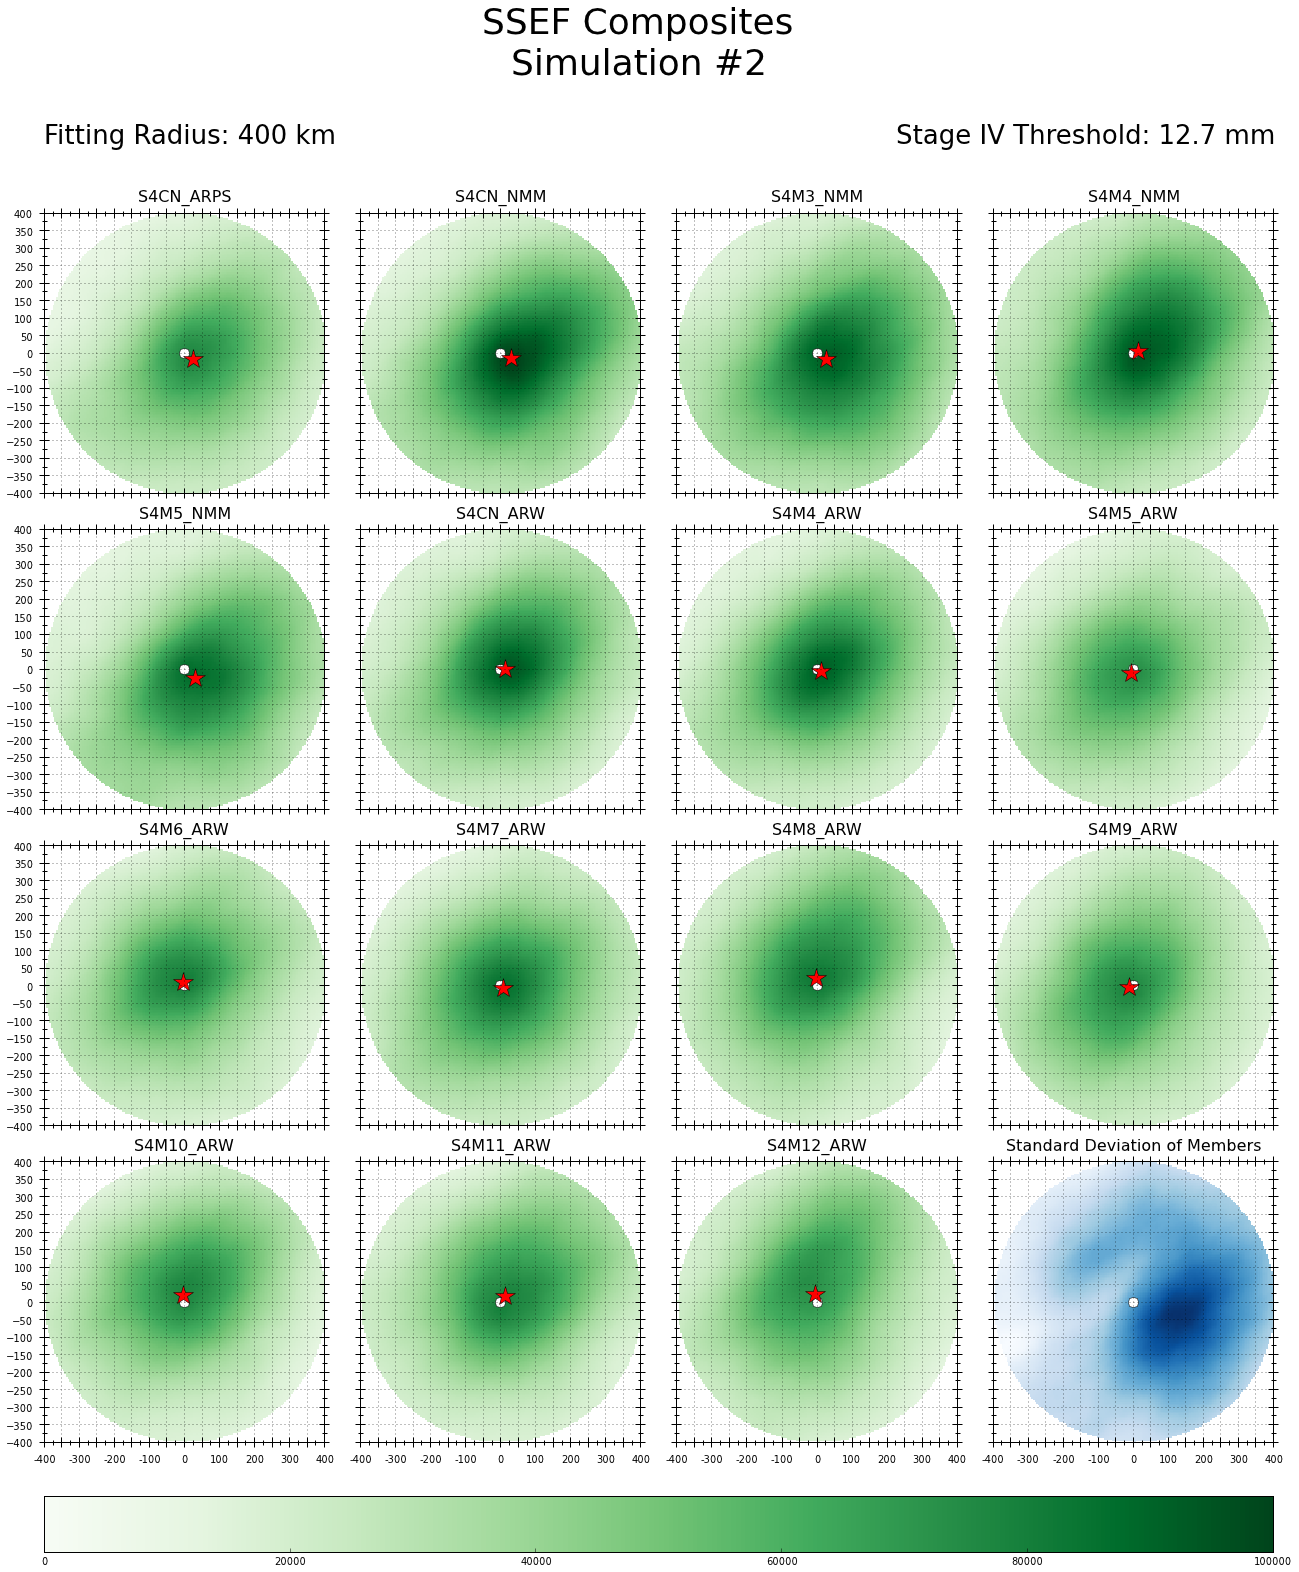
\includegraphics[width=\textwidth, height=\textheight, keepaspectratio]{%
    ./ensemble/figs/ssef_12mm_400km_composite_example.png}\\
    \caption{}
    \label{ssef-12mm-400km-composite}
\end{figure}


\clearpage
\begin{figure}[cc]
    \centering
    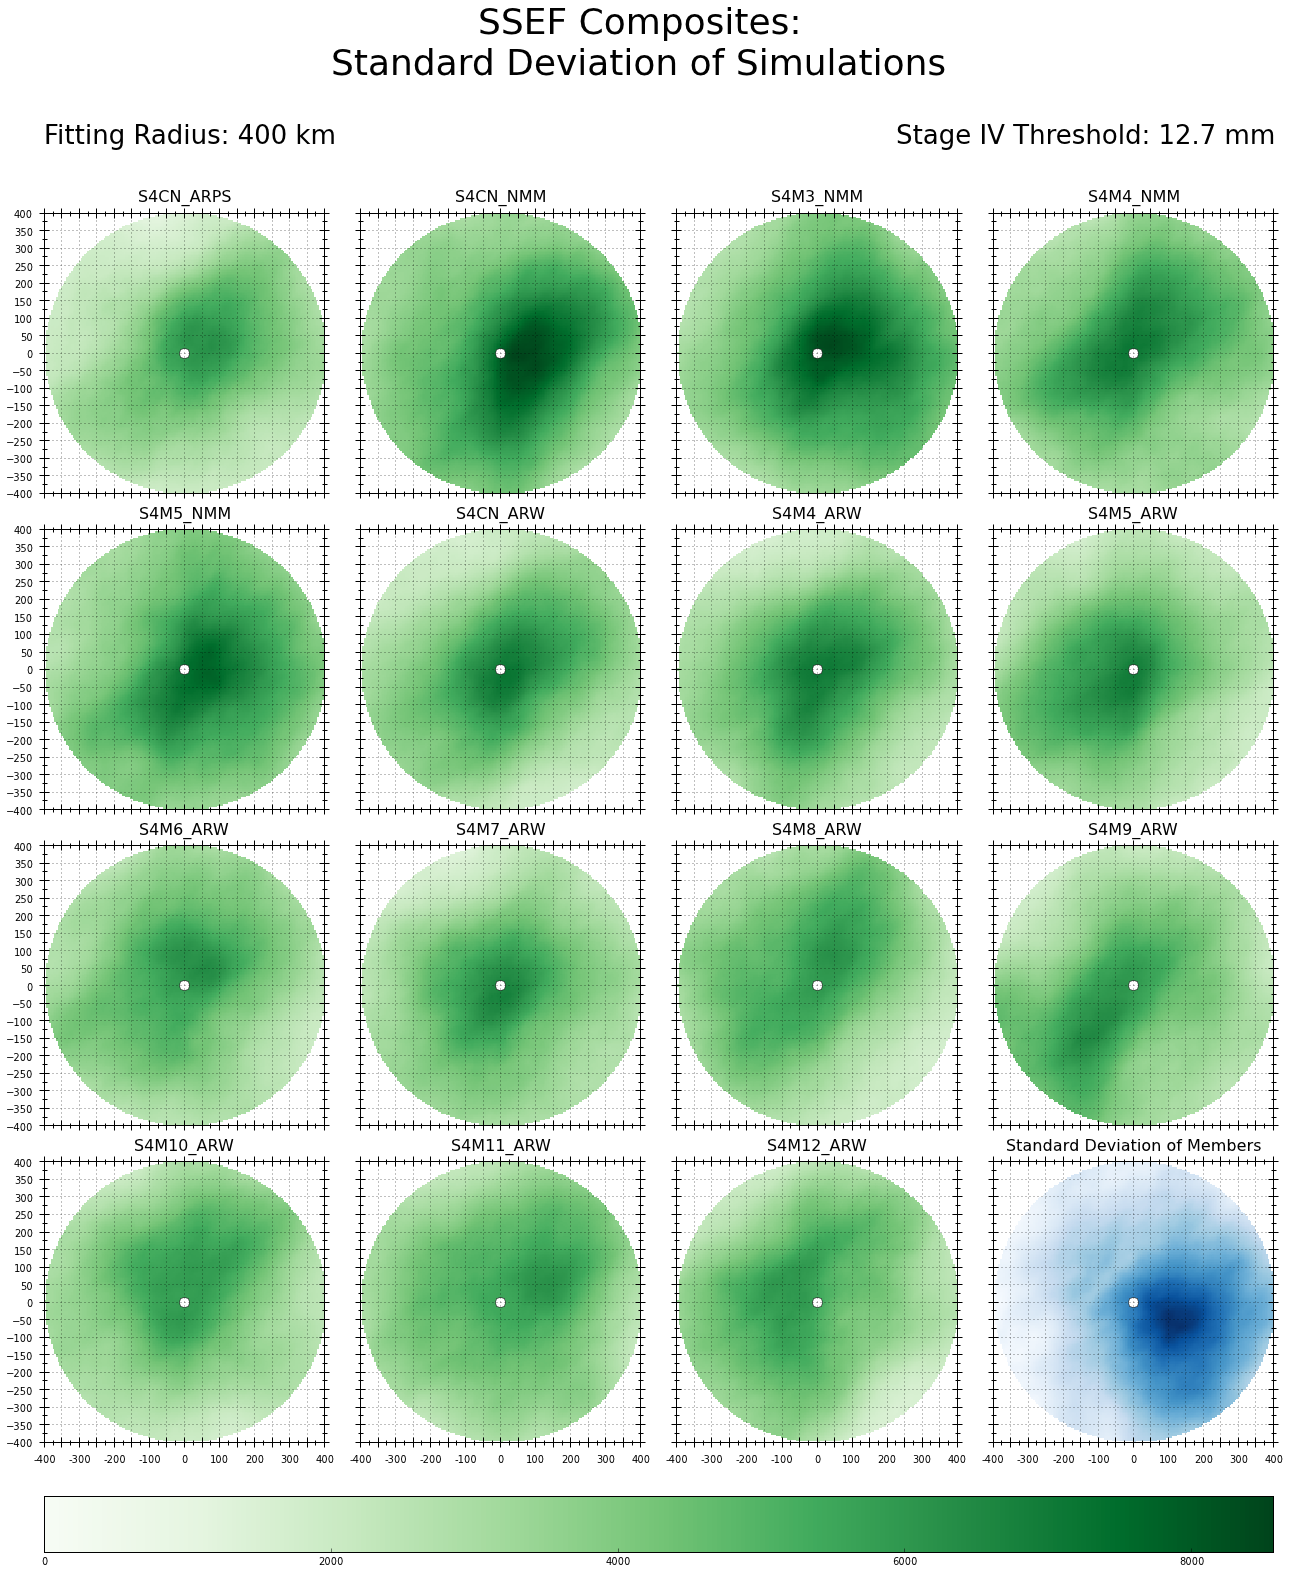
\includegraphics[width=\textwidth, height=\textheight, keepaspectratio]{%
    ./ensemble/figs/ssef_12mm_400km_composite_std.png}\\
    \caption{}
    \label{ssef-12mm-400km-std}
\end{figure}


\clearpage
\begin{figure}[cc]
    \centering
    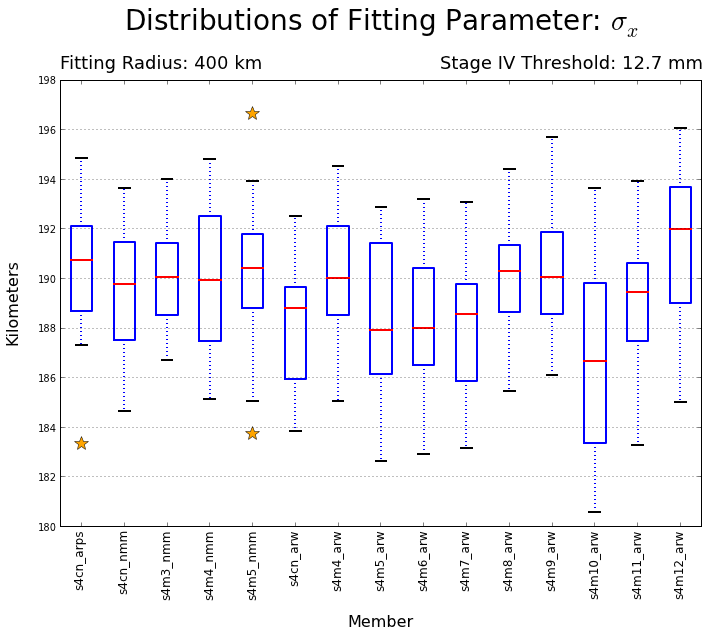
\includegraphics[width=\textwidth, height=\textheight, keepaspectratio]{%
    ./ensemble/figs/ssef_12mm_400km_sigmax.png}\\
    \caption{}
    \label{sigmax-12mm-400km-dist}
\end{figure}


\clearpage
\begin{figure}[cc]
    \centering
    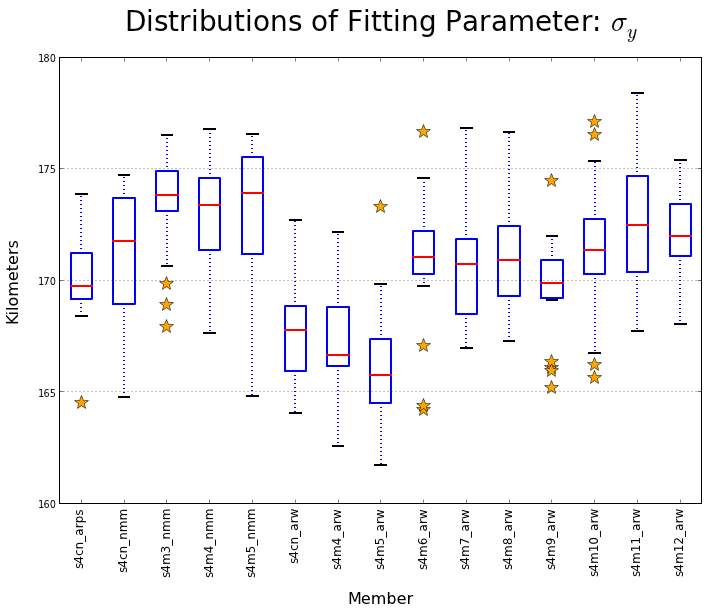
\includegraphics[width=\textwidth, height=\textheight, keepaspectratio]{%
    ./ensemble/figs/ssef_12mm_400km_sigmay.png}\\
    \caption{}
    \label{sigmay-12mm-400km-dist}
\end{figure}


\clearpage
\begin{figure}[cc]
    \centering
    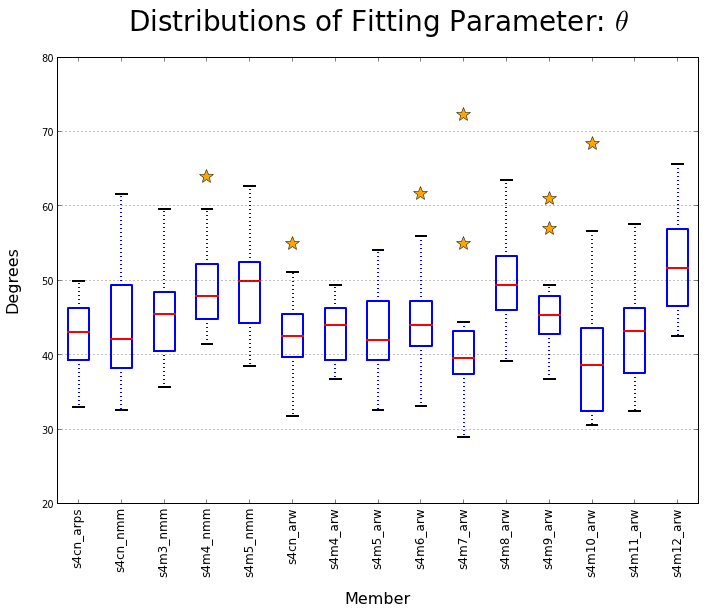
\includegraphics[width=\textwidth, height=\textheight, keepaspectratio]{%
    ./ensemble/figs/ssef_12mm_400km_theta.png}\\
    \caption{}
    \label{theta-12mm-400km-dist}
\end{figure}


\clearpage
\begin{figure}[cc]
    \centering
    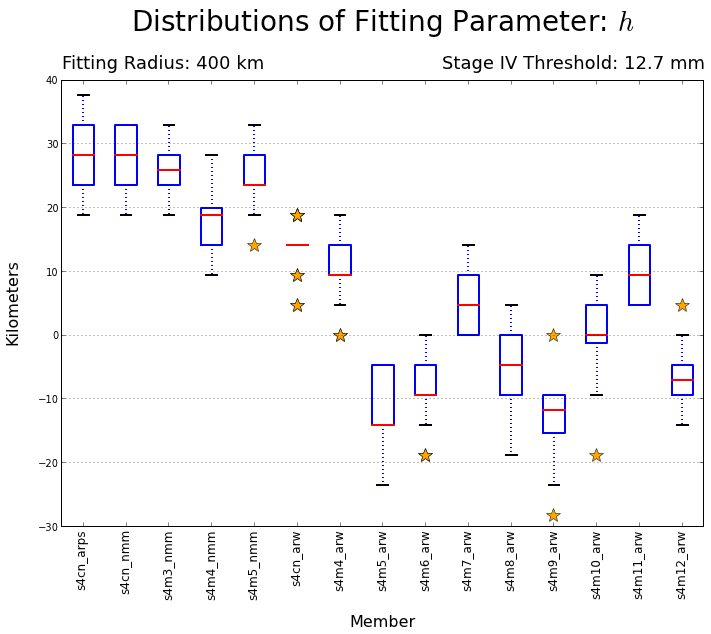
\includegraphics[width=\textwidth, height=\textheight, keepaspectratio]{%
    ./ensemble/figs/ssef_12mm_400km_h.png}\\
    \caption{}
    \label{h-12mm-400km-dist}
\end{figure}


\clearpage
\begin{figure}[cc]
    \centering
    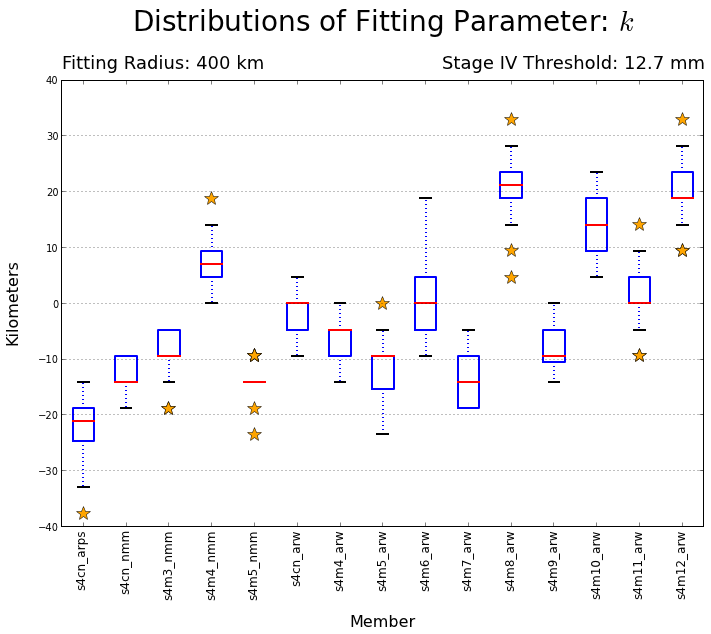
\includegraphics[width=\textwidth, height=\textheight, keepaspectratio]{%
    ./ensemble/figs/ssef_12mm_400km_k.png}\\
    \caption{}
    \label{k-12mm-400km-dist}
\end{figure}


\clearpage
\begin{figure}[cc]
    \centering
    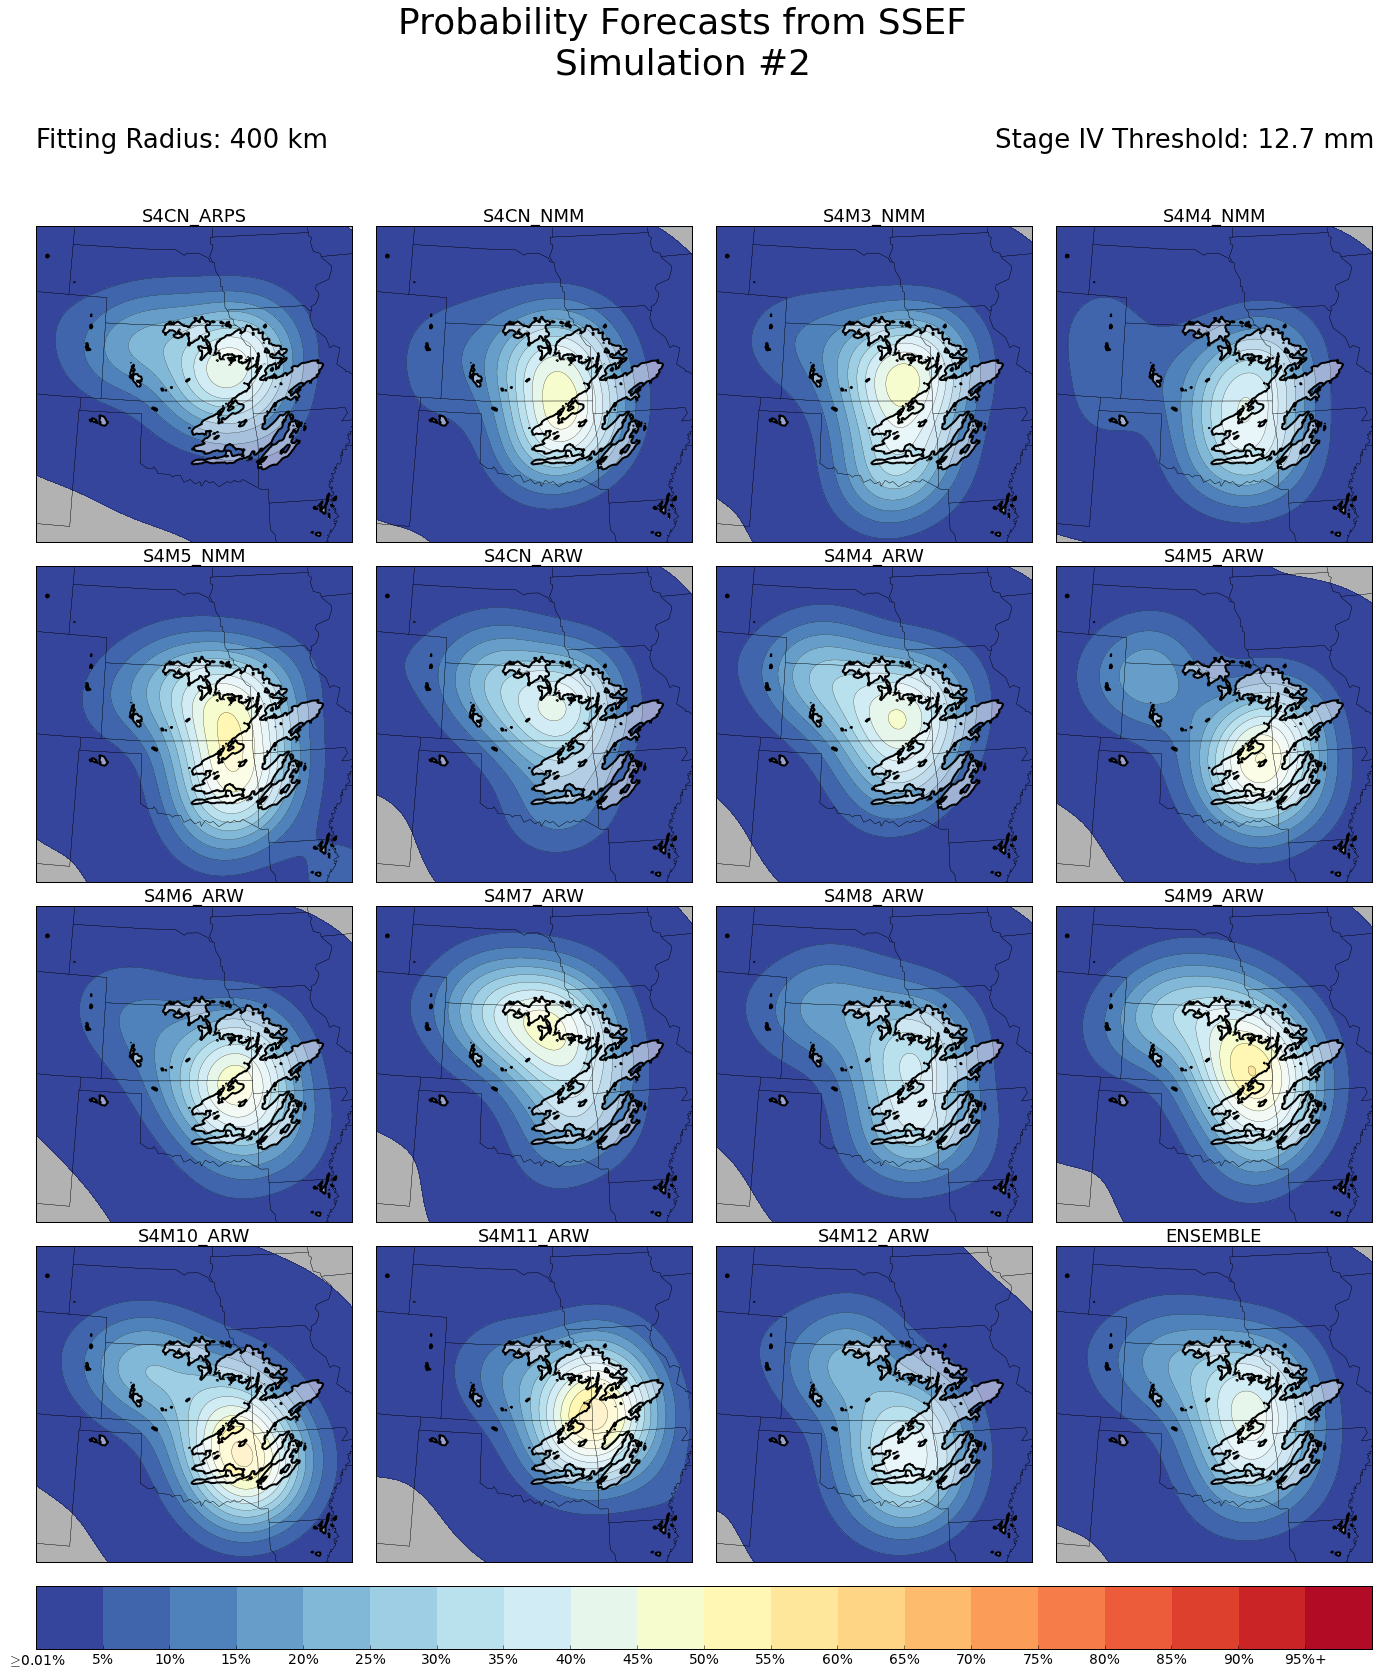
\includegraphics[width=\textwidth, height=\textheight, keepaspectratio]{%
    ./ensemble/figs/ssef_12mm_400km_example.png}\\
    \caption{}
    \label{ssef-12mm-400km-example}
\end{figure}


\clearpage
\begin{figure}[cc]
    \centering
    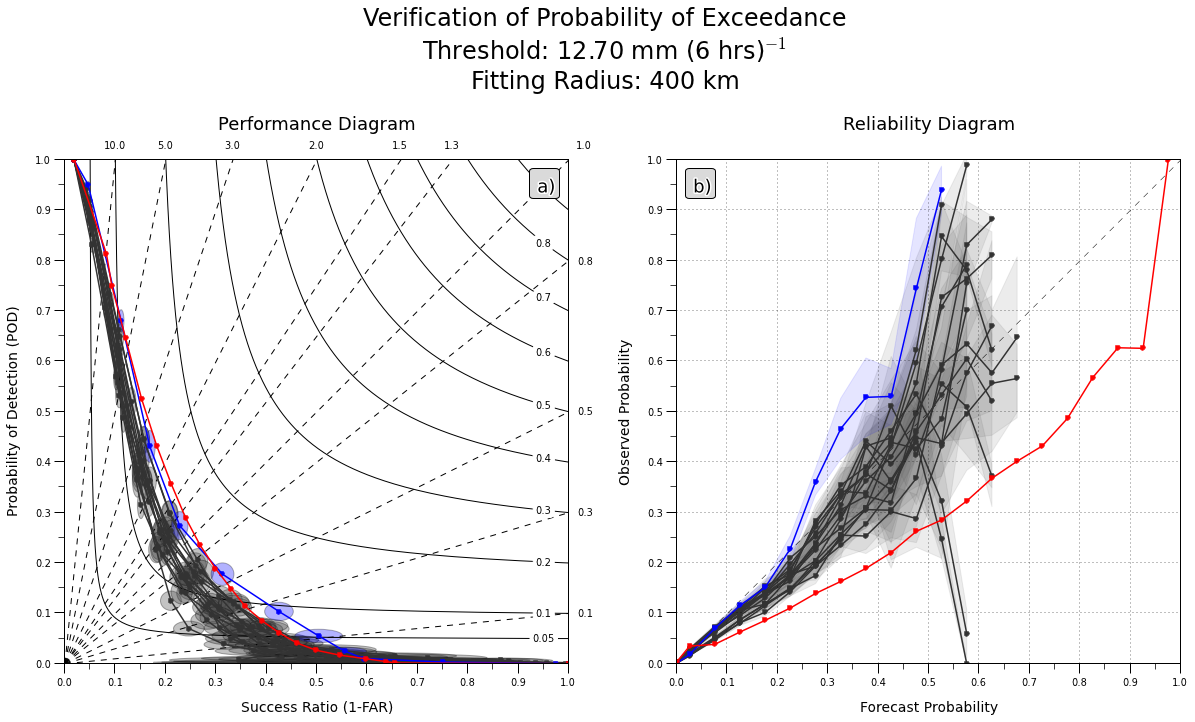
\includegraphics[width=\textwidth, height=\textheight, keepaspectratio]{%
    ./ensemble/figs/ssef_12mm_400km_verif.png}\\
    \caption{}
    \label{ssef-400km-12mm-verif}
\end{figure}

